% Document setup
\documentclass[12pt]{article}
\usepackage[margin=1in]{geometry}
\usepackage{fancyhdr}
\usepackage{lastpage}

\pagestyle{fancy}
\lhead{Richard Whitehill}
\chead{PHYS 804 -- HW \HWnum}
\rhead{\duedate}
\cfoot{\thepage \hspace{1pt} of \pageref{LastPage}}

% Encoding
\usepackage[utf8]{inputenc}
\usepackage[T1]{fontenc}

% Math/Physics Packages
\usepackage{amsmath}
\usepackage{amssymb}
\usepackage{mathtools}
\usepackage{physics}
\usepackage{siunitx}

\AtBeginDocument{\RenewCommandCopy\qty\SI}

% Enumeration/itemize
\usepackage{enumitem}
\newenvironment{parts}
{\begin{enumerate}[label=\textbf{(\alph*)},leftmargin=*,itemsep=-10pt]
}{\end{enumerate}}

% Reference Style
\usepackage{hyperref}
\hypersetup{
    colorlinks=true,
    linkcolor=blue,
    filecolor=magenta,
    urlcolor=cyan,
    citecolor=green
}

\newcommand{\eref}[1]{Eq.~(\ref{eq:#1})}
\newcommand{\erefs}[2]{Eqs.~(\ref{eq:#1})--(\ref{eq:#2})}

\newcommand{\fref}[1]{Fig.~\ref{fig:#1}}
\newcommand{\frefs}[2]{Figs.~\ref{fig:#1}--\ref{fig:#2}}

\newcommand{\tref}[1]{Table~\ref{tab:#1}}
\newcommand{\trefs}[2]{Tables~\ref{tab:#1}-\ref{tab:#2}}

% Figures and Tables 
\usepackage{graphicx}
\usepackage{float}
\usepackage[font=small,labelfont=bf]{caption}

\newcommand{\bef}{\begin{figure}[h!]\begin{center}}
\newcommand{\eef}{\end{center}\end{figure}}

\newcommand{\bet}{\begin{table}[h!]\begin{center}}
\newcommand{\eet}{\end{center}\end{table}}

% tikz
\usepackage{tikz}
\usetikzlibrary{calc}
\usetikzlibrary{decorations.pathmorphing}
\usetikzlibrary{decorations.markings}
\usetikzlibrary{arrows.meta}
\usetikzlibrary{positioning}
\usetikzlibrary{3d}
\usetikzlibrary{shapes.geometric}

% tcolorbox
\usepackage[most]{tcolorbox}
\usepackage{xcolor}
\usepackage{xifthen}
\usepackage{parskip}

\newcommand*{\eqbox}{\tcboxmath[
    enhanced,
    colback=black!10!white,
    colframe=black,
    sharp corners,
    size=fbox,
    boxsep=8pt,
    boxrule=1pt
]}

% problem-solution macros
% \usepackage{adjustbox}
\usepackage{changepage}

\newtcolorbox{probbox}[1][]{
    breakable,
    enhanced,
    boxrule=0pt,
    frame hidden,
    borderline west={4pt}{0pt}{green!50!black},
    colback=green!5,
    before upper=\textbf{Problem #1) \,},
    % \textbf{Problem #1 \ifthenelse{\isempty{#1}}{}{: #1} \\ },
    sharp corners,
    parbox=false
}

% \newtcolorbox{ProblemBox}[1][]{%
%   breakable,
%   enhanced,
%   colback=black!10!white,
%   colframe=black,
%   title={\large #1 \hfill}
% }
\newcommand{\prob}[2]{
\begin{probbox}[#1]
#2
\end{probbox}
}

\newenvironment{solution}{\begin{adjustwidth}{8pt}{8pt}}{\end{adjustwidth}}
\newcommand{\sol}[1]{
\begin{solution}
#1
\end{solution}
}
% \textbf{#1)} #2}

% Miscellaneous Definitions/Settings
\newcommand{\reals}{\mathbb{R}}
\newcommand{\integers}{\mathbb{Z}}
\newcommand{\naturals}{\mathbb{N}}
\newcommand{\rationals}{\mathbb{Q}}
\newcommand{\complexs}{\mathbb{C}}

\setlength{\parskip}{\baselineskip}
\setlength{\parindent}{0pt}
\setlength{\headheight}{14.49998pt}
\addtolength{\topmargin}{-2.49998pt}


\def\HWnum{4}
\def\duedate{October 16, 2024}



\begin{document}


\prob{1}{

Write three functions that numerically solves a first order ODE by using:
\begin{parts}
   
    \item Explicit Euler method: This is a very simple but educational exercise to get feeling about the method.

    \item Modified Euler method: The method is a bridge to methods used in particle simulations.

    \item The 5$^{\rm th}$ order Runge-Kutta-Fehlberg (RKF45).
        This is a very practical exercise leading to use a quite powerful method with an error estimate.

\end{parts}

}

\sol{

(a) The explicit Euler method is perhaps the most simple method for numerically solving a differential equation, typically introduced in a first-year calculus course.
A generic first-order ordinary differential equation takes the form
\begin{align}
    \dv{x}{t} = f(t,x(t))
,\end{align}
where $t$ is our independent variable (e.g. time) and $x(t)$ is the function of interest.
Of course, we can naively approximate the derivative at $t$ as the slope of the secant line between $t$ and $t + h$, where $h$ is small step.
Doing, so we have
\begin{align}
    \dv{x}{t} \approx \frac{x(t + h) - x(t)}{h} = f(t,x(t))
.\end{align}
From this, we can approximate $x(t+h)$ by having some initial value for $x(t)$ through
\begin{align}
    x(t + h) \approx x(t) + h f(t,x(t))
,\end{align}
and therefore, we can define a recursive sequence of approximations by first specifying an initial condition $x(t_0) = x_0$ and computing
\begin{align}
    x_{n+1} = x_{n} + h f(t_n,x_{n})
,\end{align}
where $t_{n} = t + nh$ and $x_{n} = x(t_{n})$, until we reach some final time $t_1$.
Typically, the step-size is derived by specifying the number of steps $N$ between $t_0$ and $t_1$ as $h = (t_1 - t_0) / N$.


(b) As one probably knows from a differential equations class, the Euler method is only $\mathcal{O}(h^2)$ accurate, modulated by the size of the second-derivative of $x$, and hence suffers from some significant systematic defects unless our step size $h \ll (t_1 - t_0)$ (i.e. $N \gg 1$).
There are two ways to make these errors smaller.
Firstly, we can devise methods such that the local truncation error of order $\mathcal{O}(h^{n})$ is such that $n$ is larger, or secondly, we can devise a method which adjusts the size of $h$ at each step.
A first improvement to Euler's method is the modified Euler (or Heun's) method, which aims to mitigate the error as follows.
If we adopt notation consistent with the general class of Runge-Kutta methods, we define our recursive sequence as follows:
\begin{align}
    k &= x_{n} + h f(t_{n},x_{n}) \\
    x_{n+1} &= x_{n} + \frac{h}{2} \Big[ f(t_{n},x_{n}) + f(t_{n+1},k) \Big]
.\end{align}
Indeed, by averaging the slopes in the above way, we increase by one power of $h$ the local truncation error to $\mathcal{O}(h^3)$.


(c) As alluded to in part (b) another way to obtain more accurate numerical schemes is to devise one such that our step size is adjusted at each step so that at each step our prescribed error is less than some tolerance.
In the RKF45 scheme, we use the 5$^{\rm th}$ order Runge-Kutta scheme for our recursive sequence.
Generically, an $N^{\rm th}$ Runge-Kutta method is given by
\begin{align}
\begin{aligned} 
    k_1 &= h f(t_{n},x_{n}) \\
    k_2 &= h f(t_{n} + b_{1} h, x_{n} + A_{11} k_1) \\
    &\vdots \\
    k_{N+1} &= h f(t_{n} + b_{N} h, x_{n} + A_{Ni} k_{i}) \\
    x_{n+1} &= x_{n} + h c_{i}^{(N)} k_{i}
,\end{aligned}
\end{align}
where the coefficients $b_{i}$, $c_{i}^{(N)}$, and $A_{ij}$ are method-specific.
Note that for brevity we utilize Einstein summation convention where repeated indices are summed implicitly.
Although we do not have the exact solution with which to compute an error, we can define an error as the difference between the $N^{\rm th}$ and $(N - 1)^{\rm th}$ RK method:
\begin{align}
    e_{n+1} = \Big[ c_{i}^{(N)} - c_{i}^{(N-1)} \Big] k_{i}
,\end{align}
where $d_{i}$ is again a vector of coefficients dependent on the method.
With this estimate, if our error $e_{n+1} > \epsilon$, where $\epsilon$ is some tolerance, then we redefine our step size as
\begin{align}
    h = \min\{ 0.9 h (\epsilon/|e_{n+1}|)^{1/(N+1)}, 0.5 h \}
\end{align}
and repeat the step.
Alternatively, if $e_{n+1} \leq \epsilon$, then we accept the step and redefine our step size as
\begin{align}
    h = \min\{ 0.9 h (\epsilon/|e_{n+1}|)^{1/(N+1)},2h \}
.\end{align}

Typically, the coefficients are specified by a Butcher tableau.
For the RKF45 method, the Butcher tableau is as follows:
\begin{table}[H]
    \centering
    \begin{tabular}{c|cccccc}
        1/4 & 1/4 &  &  &  &  & \\
        3/8 & 3/32 & 9/32 &  &  & &  \\
        12/13 & 1932/2197 & -7200/2197 & 7296/2197 & & &  \\
        1 & 439/216 & -8 & 3680/513 & -845/4104 & & \\
        1/2 & -8/27 & 2 & -3544/2565 & 1859/4104 & -11/40  & \\
        \hline
         & 16/135 & 0 & 6656/12825 & 28561/56430 & -9/50 & 2/55 \\
         & 25/216 & 0 & 1408/2565 & 2197/4104 & -1/5 & 0
    \end{tabular}
\end{table}


}

\inputpython{main.py}


\prob{2}{

Solve numerically following ODEs (employing all three methods), and study the effect of step size by calculating the relative error either by comparing with analytic solution or with RKF45 (if analytic solution is not attainable).

\begin{parts}

\item $x' = x + e^{-t}$ with $x(0) = 0$ in the interval $t \in [0,1]$.

\item $x' = x + 2 \cos{t}$ with $x(0) = 1$ in the interval $t \in [0,1]$.

\item $x' = t x^2$ with $x(0) = 1$ in the interval $t \in [0,1]$.

\item $x' = 1.5 \sin{2x} - x \cos{t}$ with $x(0) = 1$ in the interval $t \in [0,10]$.
    
\end{parts}

}

\sol{

We can obtain analytic solutions for parts (a) -- (c), which are as follows:
\begin{align} 
    &(a)~\mbox{--}~x(t) = \sinh{t} \\
    &(b)~\mbox{--}~x(t) = 2 e^{t} + \sin{t} - \cos{t} \\
    &(c)~\mbox{--}~x(t) = \frac{2}{2 - t^2}
.\end{align}
Numeric results are displayed in \fref{prob2}.
Across the board, we can see that the RKF45 and modified Euler methods perform quite well at a step size of $h = 0.1$, being within 1\% of the analytic values, while the Euler method tends to start diverging from the exact or RKF45 solution closer to $t = 1$, being as much as roughly 15\% from the analytic result in part (c).


\begin{figure}[H]
    \centering
    \centerline{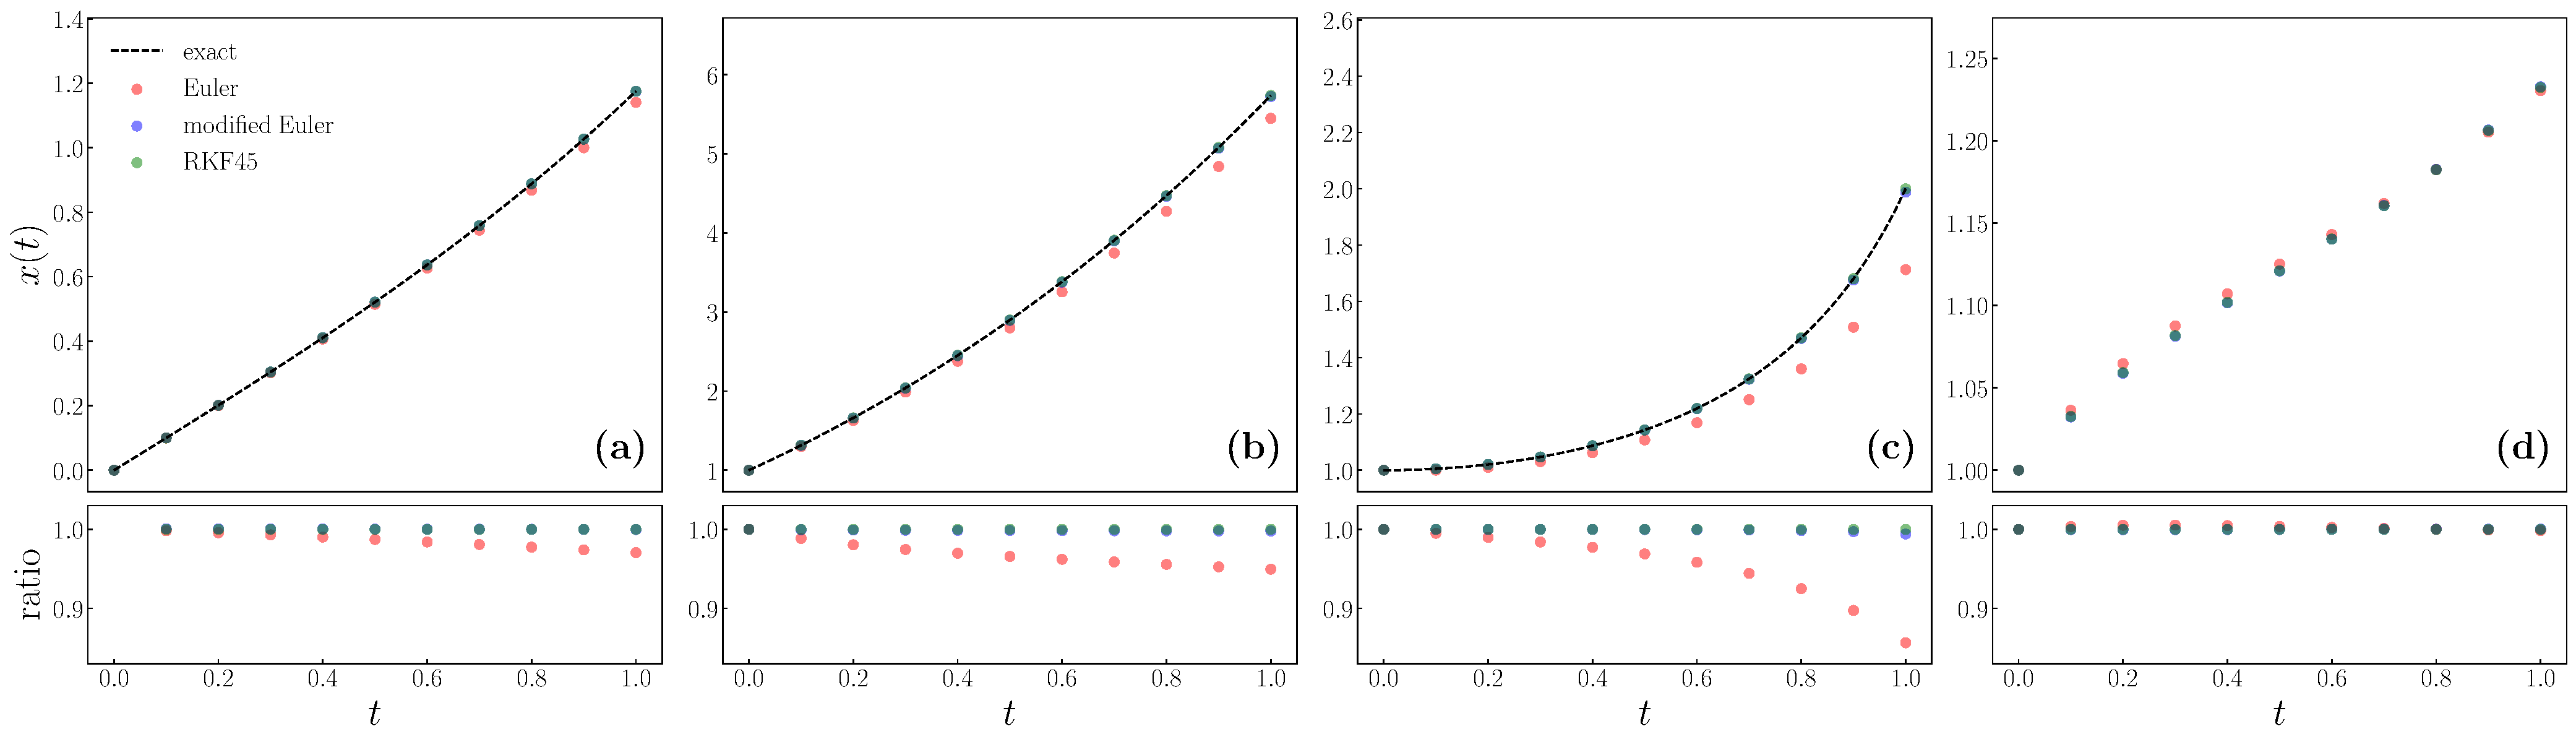
\includegraphics[width=0.9\paperwidth]{prob2.pdf}}
    \caption{In the top row of panels, a comparison of the exact (when an analytic solution is possible to obtain), Euler, modified Euler, and RKF45 (without adaptive step sizes) solutions to the respective differential equation given in problem 2 is shown, and in the lower panel, we plot the ratio of the results of the numerical scheme to the value provided by the exact solution (or RKF45 result when  an analytic solution is notavailable).}
    \label{fig:prob2}
\end{figure}

\inputpython{prob2.py}

}


\prob{3}{

Using the error estimation in the 5$^{\rm th}$ order Runge-Kutta-Fehlberg method, you can upgrade your code to include adaptive step control.
Apply your upgraded code to problem 2.4.
Report your observations when you start either with a very small step or very large step and compare with the results when you do not employ adaptive step size.

}

\sol{

From \fref{prob3}, we can see the performance of our RKF45 with static and adaptive step sizes for three different initial step sizes: $10^{-2},10^{-1},~{\rm and}~1$.
It is clear that the solutions cannot be properly reconstructed with one static step, but it is not too bad when we take 10 steps and certainly a more resolved construction when we take 100 static steps.
When one permits the step-size to change with a tolerance of $\epsilon = 10^{-4}$, we can see that a step size of about $1/6$ is approximately optimal across the time interval to construct the solution, and therefore there is only a slight adjustment of the step sizes when $h_0 = 0.1$.
When $h_0 = 1$, the first step is not accepted until a much smaller step of roughly $h = 0.3$ is attained and decrease subsequently.
On the other hand, while the steps are accepted initially for $h_0 = 0.01$, the code makes the subsequent steps larger because such small steps are not necessary to accurately produce the result.

\begin{figure}[H]
    \centering
    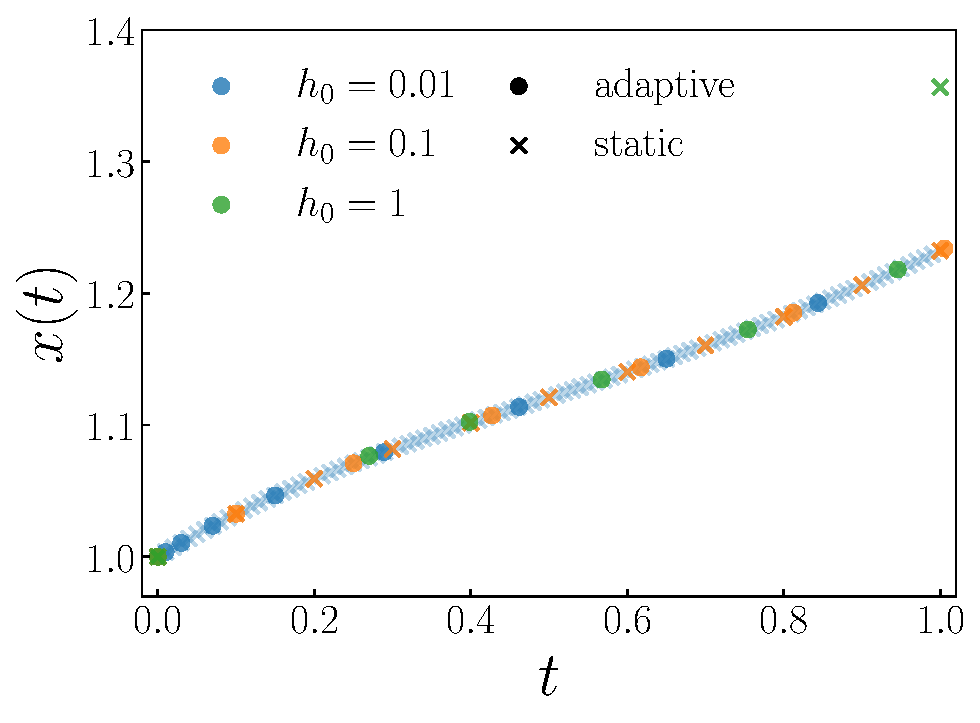
\includegraphics[width=0.7\textwidth]{prob3.pdf}
    \caption{Comparison of solutions using the RKF45 method with and without adaptive step sizes for an array of initial step sizes $h_0$.}
    \label{fig:prob3}
\end{figure}


\inputpython{prob3.py}

}


\prob{4}{

\begin{parts}

\item Under certain conditions the rate of change of the temperature of a body, immersed in a medium whose temperature (kept constant) differs from it, is proportional to the difference in termperature between it and the medium.
    In mathematical symbols, this statement is written as
    \begin{align}
        \dv{T}{t} = -k(T - T_{M})
    ,\end{align}
    where $k > 0$ is a proportionality constant, $T$ is the temperature of the body at any time $t$, and $T_{M}$ is the constant temperature of the medium.
    Let's say you have a cup of coffee at $90 ^{\circ}{\rm C}$ initially ($T_0 = 90$) and its placed in a room where the temperature is $20 ^{\circ}{\rm C}$ initially ($T_{M} = 20$).
    The constant $k$ is given as 0.05 (per minute).
    We want to find the temperature of the coffee after 10 minutes.
    Think, how can you test your code?
   
\item A projectile of mass $m = 1~{\rm kg}$ is thrown vertically upward from the ground with an initial velocity $v_0 = 20~{\rm m/s}$.
    The projectile is the subject to linear air resistance so that the force of air resistance is given $f_{d} = -bv$ with $b = 1~{\rm kg/s}$.
    Find its velocity as a function of time.
    For how long will it rise?

    Note: Newton's second law reads
    \begin{align}
        m \dv{v}{t} = - mg - bv
    ,\end{align}
    where $m$ is the mass, $g$ is the free-fall acceleration, and $b$ is the linear drag coefficient.
    Think, how can you test your code?

\item A projectile of mass $m = 1~{\rm kg}$ is thrown vertically upward from the ground with an initial velocity $v_0 = 20~{\rm m/s}$.
    The projectile is the subject to linear air resistance so that the force of air resistance is given $f_{d} = -c v^2$ with $c = 0.1~{\rm kg/m}$.
    Find its velocity as a function of time.
    For how long will it rise?

    Note: Newton's second law reads
    \begin{align}
        m \dv{v}{t} = - mg - c v^2
    ,\end{align}
    where $m$ is the mass, $g$ is the free-fall acceleration, and $b$ is the linear drag coefficient.
    Think, how can you test your code?

\end{parts}

}

\sol{

(a) The exact solution to the differential equation is
\begin{align}
    T(t) = T_{M} + (T_0 - T_{M}) e^{-k t}
,\end{align}
so 
\begin{align}
    T(10~{\rm min}) \approx 62.457^{\circ}{\rm C}
.\end{align}
With the RKF45 method with $\epsilon = 10^{-4}$, we obtain $T(10) \approx 62.496^{\circ}{\rm C}$.
Howver, with $\epsilon = 10^{-6}$, we have $T(10) \approx 62.458^{\circ}{\rm C}$.
Although our result is quite accurate in both cases, a lesson to be wary of is that the error can propagate to a noticeable and perhaps significant level over a few steps, so one must always balance computational efficiency and accuracy.

\begin{figure}[H]
    \centering
    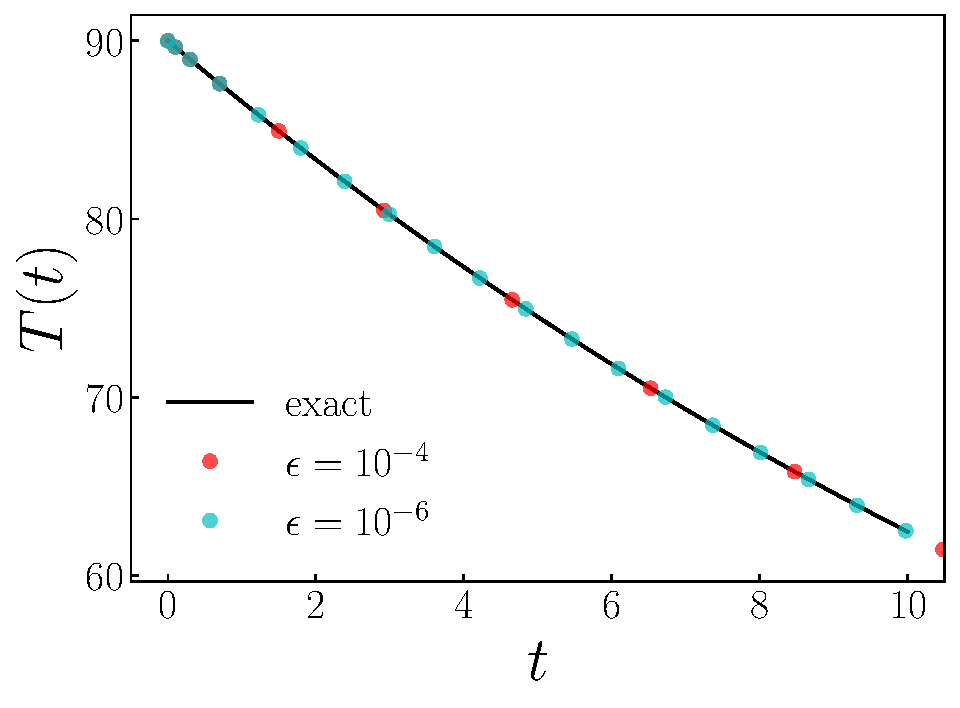
\includegraphics[width=0.7\textwidth]{prob4a.pdf}
    \caption{Results using RKF45 method to solve Newton's law of cooling equation with the prescribed initial conditions and physical constants.}
    \label{fig:prob4a}
\end{figure}

\inputpython{prob4a.py}


(b) The analytic solution to this differential equation is
\begin{align}
    v(t) = ( v_0 + v_{t} ) e^{-t/\tau} - v_{t}
,\end{align}
where $v_{t} = mg/b$ and $\tau = m/b$ are the terminal speed and characteristic damping time of our system.
Solving this equation for $T$ where 
\begin{align}
    v(T) = 0 \Rightarrow T = \tau \ln(1 + \frac{v_0}{v_{t}}) = 1.112~{\rm s}
\end{align}
for the input physical parameters and initial condition.

\begin{figure}[H]
    \centering
    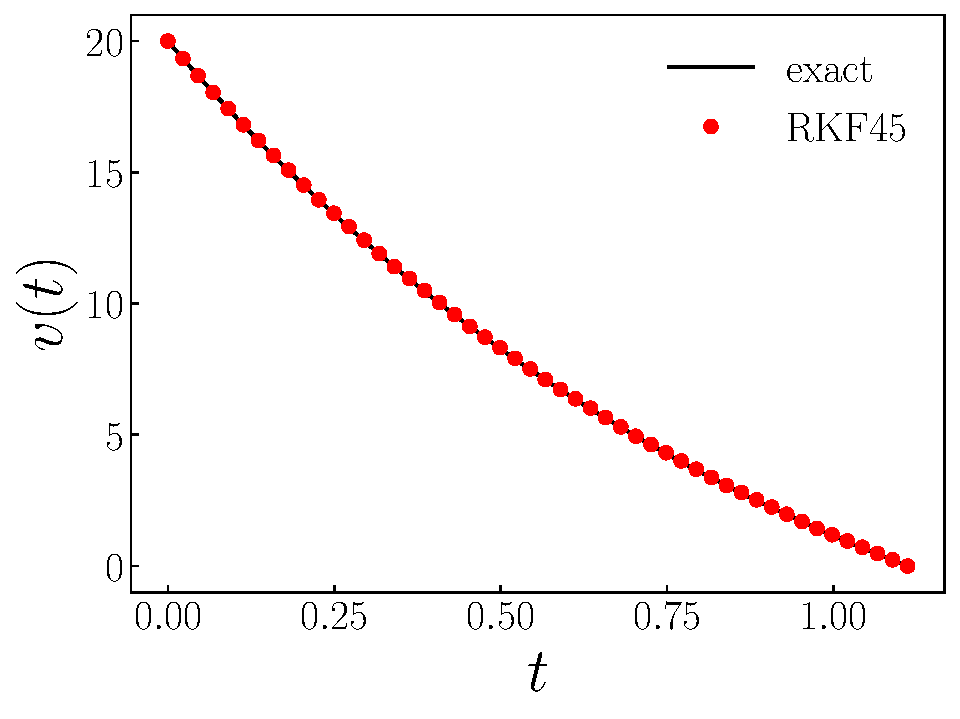
\includegraphics[width=0.7\textwidth]{prob4b.pdf}
    \caption{Results using the RKF45 method to solve Newton's 2$^{\rm nd}$ law for a vertically launched projectile under a linear drag force with initial velocity $v_0 = 20~{\rm m/s}$.}
    \label{fig:prob4b}
\end{figure}

\inputpython{prob4b.py}


(c) In this case, the analytic solution (for purely upward motion -- the sign is flipped on the drag force when the projectile moves down) is
\begin{align}
    v(t) = v_{c} \tan\Bigg[ \arctan(\frac{v_0}{v_{c}})  - \frac{t}{\tau} \Bigg]
,\end{align}
where $v_{c} = \sqrt{m g / c}$ and $\tau = v_{c} / g$.
Solving for the time $T$ where the velocity $v(T) = 0$ we find
\begin{align}
    T = \tau \arctan(\frac{v_0}{v_{c}}) \approx 1.122~{\rm s}
\end{align}
with the physical parameters and initial speed as given.

\begin{figure}[H]
    \centering
    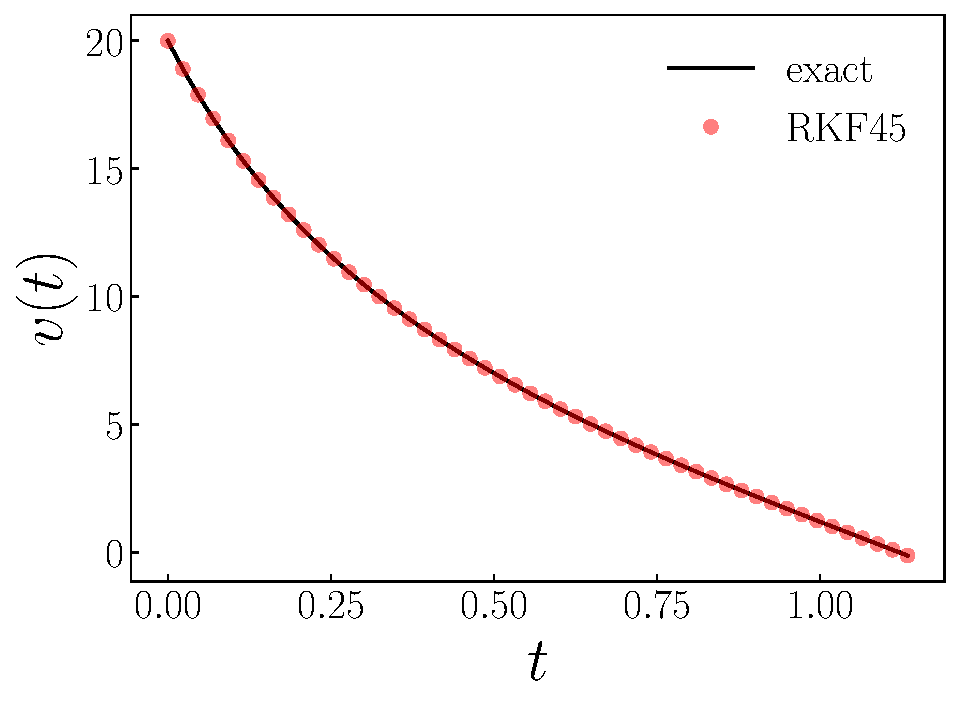
\includegraphics[width=0.7\textwidth]{prob4c.pdf}
    \caption{Results using the RKF45 method to solve Newton's 2$^{\rm nd}$ law for a vertically launched projectile under a quadratic drag force with initial velocity $v_0 = 20~{\rm m/s}$.}
    \label{fig:prob4c}
\end{figure}

\inputpython{prob4c.py}

}

    
\end{document}
